% v4 Results: the dimension axis (split out of s4_b_reconstruction at the
% Session 37 Stage 3 restructure; probe-dilution control accompanies the
% dimension figure per the locked rule). All numbers through the macros
% pipeline.

\subsubsection{How small the state can be}
\label{sec:res_dimension}

The dimension axis splits into two tiers, and the split is the paper's
compression statement (figure~\ref{fig:dimrace}a). At $d = 4$ the
predictive families read the peak loads through a linear probe at
\PoneLowdJepa{} for the \PredState{} lineage against \PoneLowdFukami{} for the
reconstructive baseline, three seeds each with non-overlapping ranges; the
lift-focused lineage forecast through the \DirectFC{} rather than the
autoregressive predictor is close to dimension-insensitive on the peaks, where
the \PredState{} lineage declines with $d$ (figure~\ref{fig:dimrace}a). A
four-coefficient lift-critical state is therefore viable. The wake state is not
compressible to it: the decoded structural fidelity of the same lineage rises
monotonically with dimension (figure~\ref{fig:dimrace}c), so the wake-bearing
state needs $d \geq 16$ while the lift saturates by $d \approx 4$ to $8$.

The probe-dilution control disciplines how the first tier may be read
(figure~\ref{fig:dimrace}b). A multilayer probe nearly equalises every
dimension (from \PdMlpDFour{} at $d = 4$ to \PdMlpDThirtyTwo{} at
$d = 32$ on the \TestSplit{} set): the lift information in the state is
approximately unchanged over the tested dimensions, and small states do not
know more. What changes with
dimension is linear accessibility. The best four coordinates of a larger
state recover only \PdBestFourDEight{} to \PdBestFourDThirtyTwo{} through
a linear read-out, so the code is distributed rather than diluted, and the
$d = 4$ advantage is exactly that four coordinates are what a linear
probe, a filter gain, or a controller reads directly. The precise form of
the two-tier claim is therefore: compact and linear at $d = 4$,
distributed and partly nonlinear above.

\begin{figure}
  \centering
  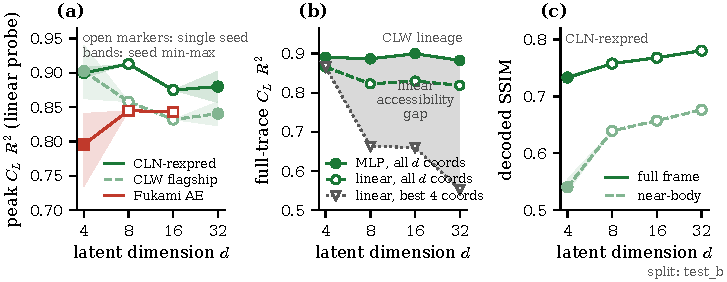
\includegraphics[width=\linewidth]{sections/figures/results/fig_dimension_race_v4.pdf}
  \caption{The dimension axis on the \TestSplit{} set. (a)~Peak-region lift $R^2$
  (linear probe) against latent dimension for the three lineages; shaded
  bands are three-seed min-max ranges, open markers single seeds.
  (b)~The probe-dilution control: a multilayer probe is flat in $d$ while
  the best-four-coordinate linear probe falls, so the $d = 4$ advantage is
  linear accessibility of a distributed code, not information.
  (c)~Decoded SSIM (Wang convention, \S\ref{sec:methods_protocol}) of the
  same lineage rises with $d$: the wake tier is not compressible.}
  \label{fig:dimrace}
\end{figure}
